\chapter{Architekturschichten}\label{ch:arrchitekturschichten}
Im Folgenden wird die Architektur der Applikation genauer beschrieben. Dabei liegt das Augenmerk 
auf der Struktur, dem Verhalten und der Verteilung der einzelnen Komponenten in der Architektur.

%Einzelne Unterkategorien werden ergänzt, wenn die Implementierung der Applikation voran schreitet.

\section{Strukturschicht}\label{sec:strukturschicht}
% ,angle=90,origin=c

% \subsection{Backend} % No need for a subsection if there is only one
In diesem Abschnitt ist die Struktur des Backends beschrieben.

\begin{figure}[H]
    \centering
    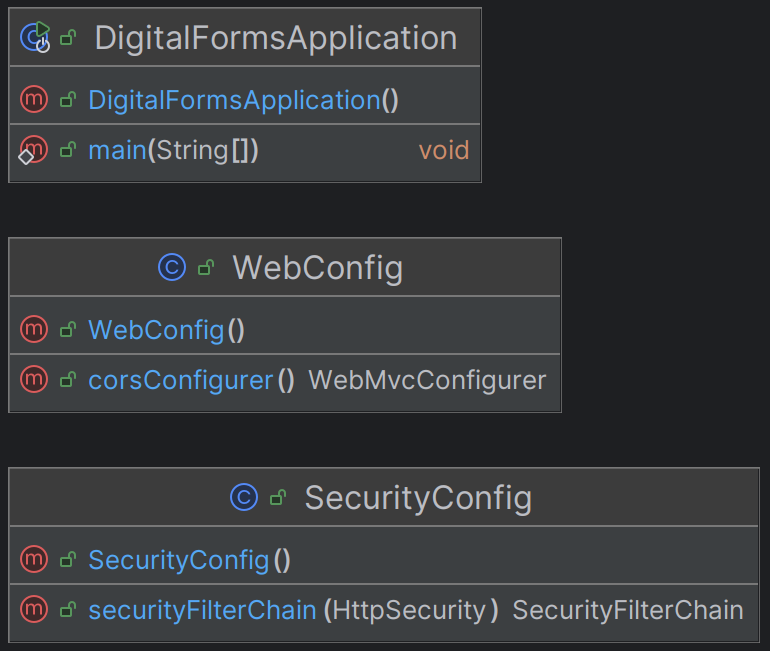
\includegraphics[width=15cm]{images/classDiagrams/Config}
    \caption{Backend Spring Boot Configuration}\label{fig:Backend-Spring-Boot-Configuration}
\end{figure}

\refa{fig:Backend-Spring-Boot-Configuration} zeigt die Konfiguration des Spring Boot Projekts.
Dabei startet "DigitalFormsApplication" das Projekt, "WebConfig" konfiguriert CORS Einstellungen und "SecurityConfig"
Konfiguriert die Zugriffsoptionen auf die Endpunkte.

\begin{figure}[H]
    \centering
    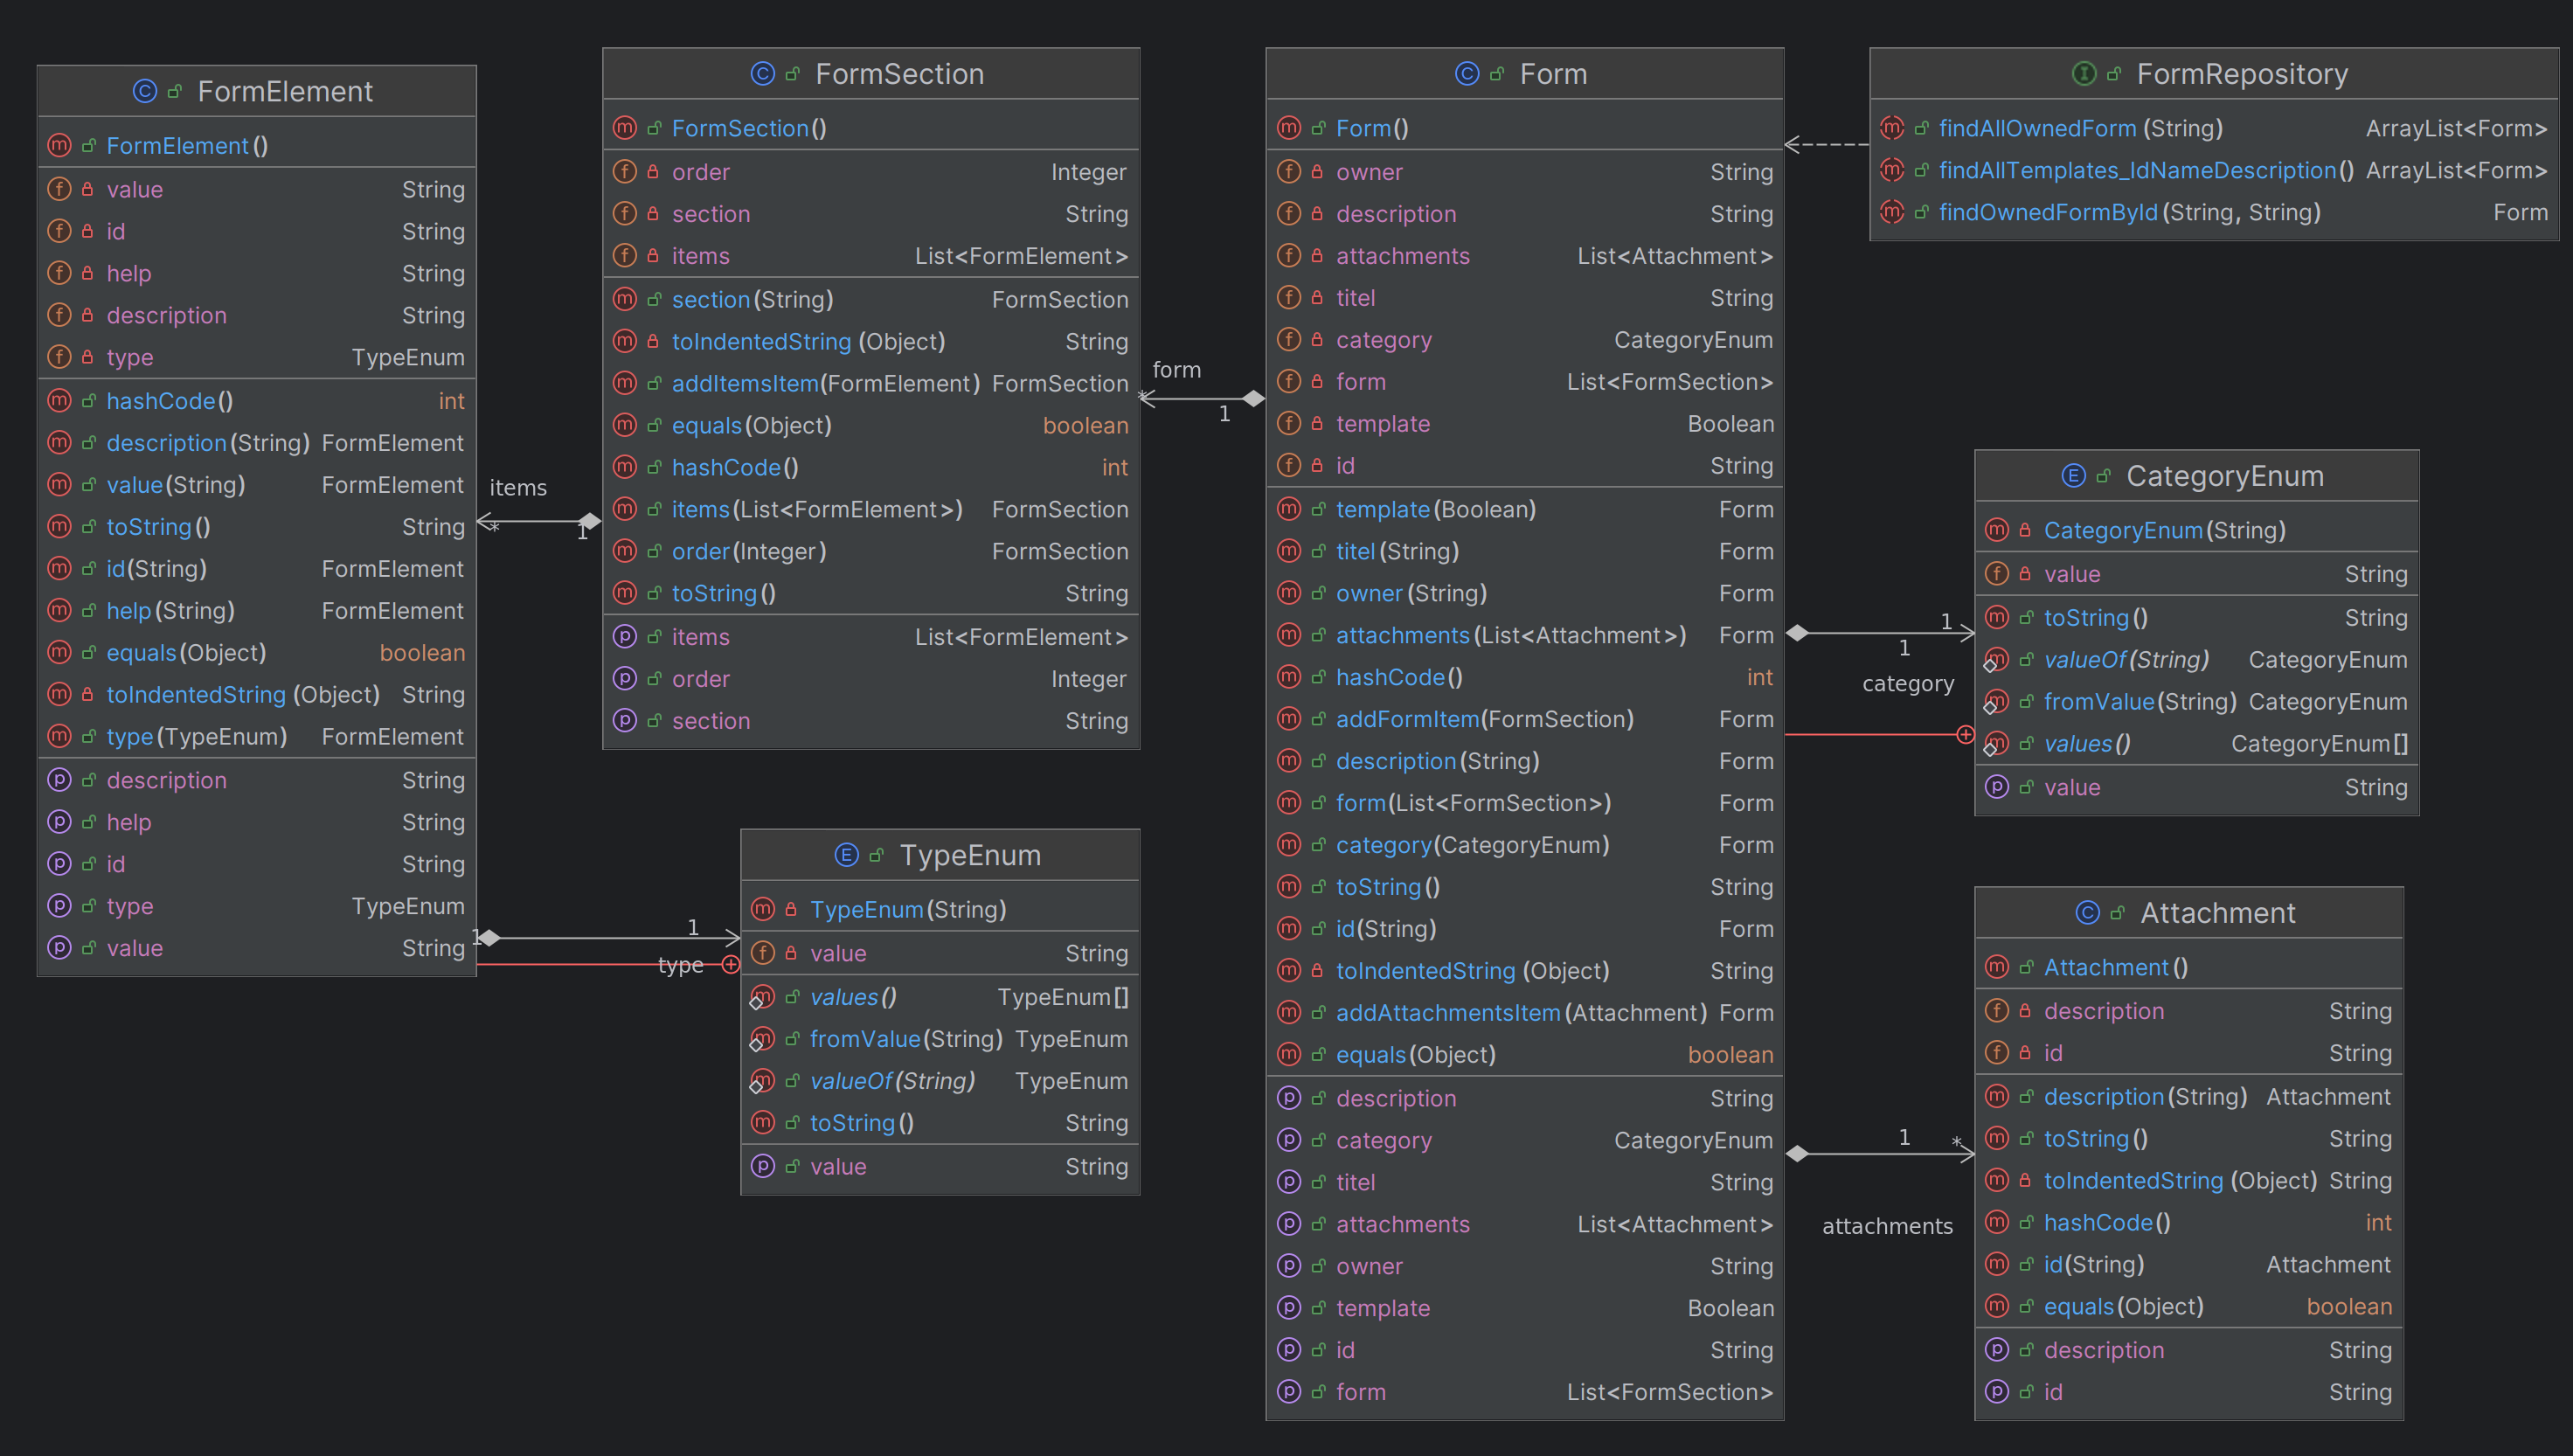
\includegraphics[width=20cm,angle=90,origin=c]{images/classDiagrams/FormRepository}
    \caption{Backend Datenmodell}\label{fig:backendclass-diagram}
\end{figure}

\refa{fig:backendclass-diagram} zeigt den detailarten Aufbau des Datenbankmodells.
Dabei dient "FormRepository" als Schnittstelle für die Datenbank.
Die Objektmodelle werden durch die OpenAPI Spezifikation automatisch generiert.

\begin{figure}[H]
    \centering
    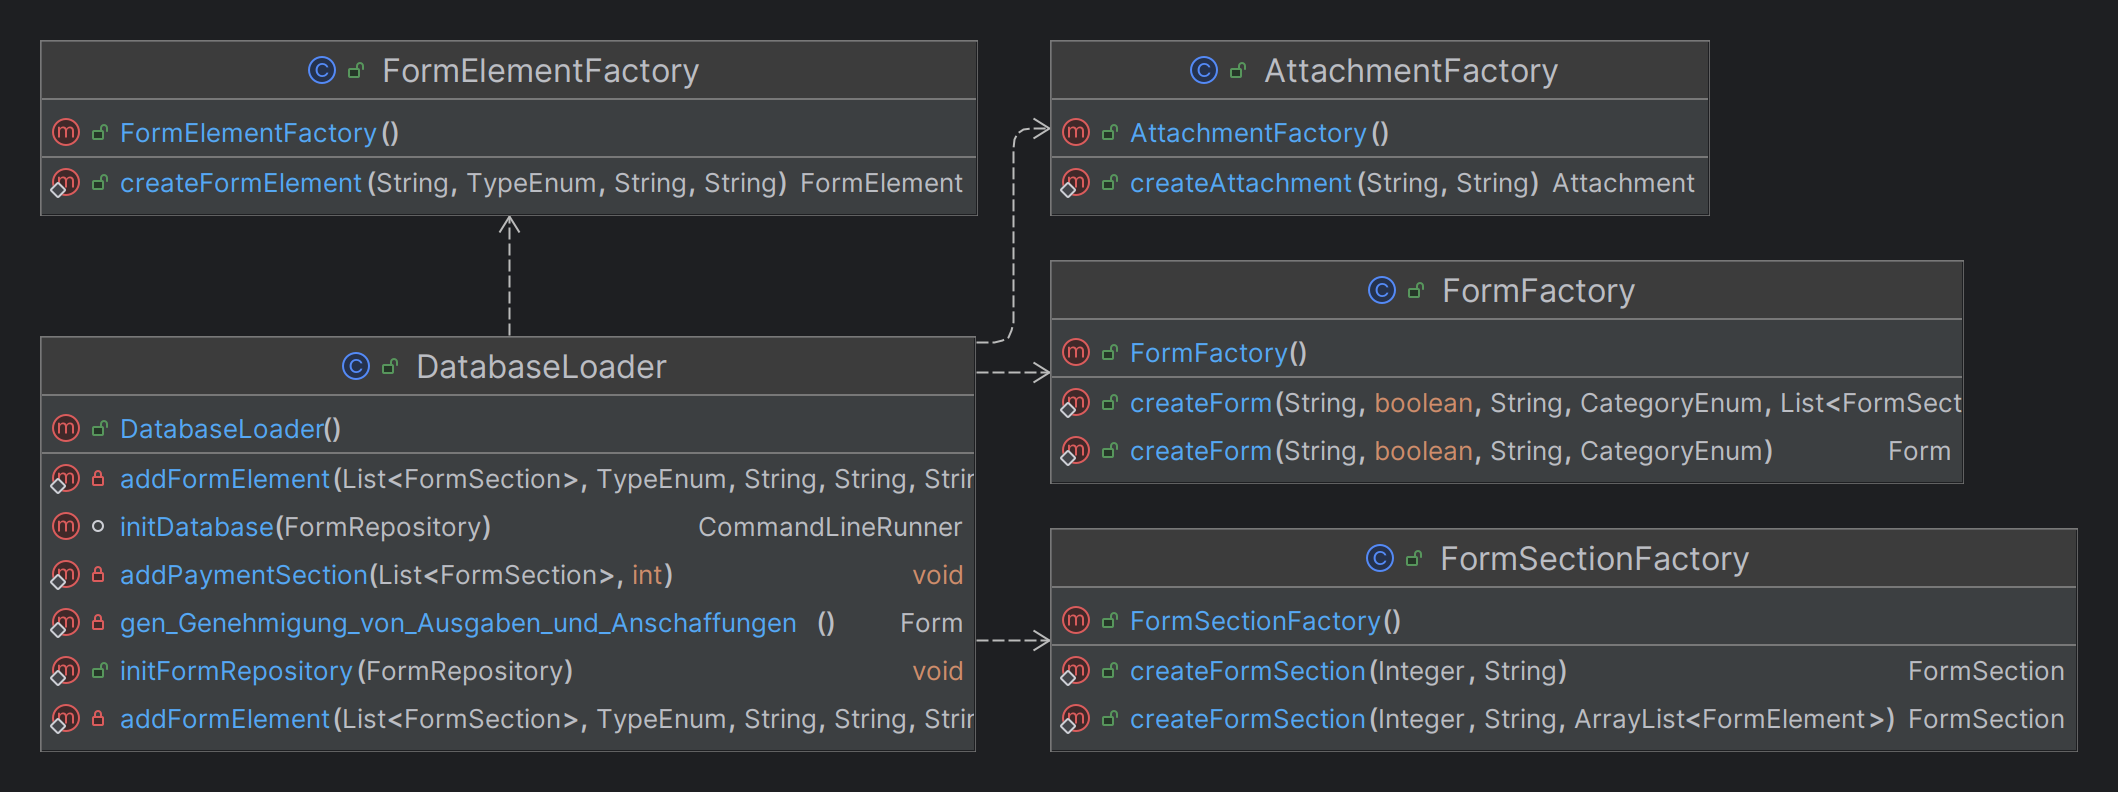
\includegraphics[width=15cm]{images/classDiagrams/DatabaseLoader}
    \caption{Backend Datenbank Init und Factorys}\label{fig:backend-gen-class-diagram}
\end{figure}

Um die Datenbank mit Elementen zu initialisieren, wird der "DatabaseLoader" aus \refa{fig:backend-gen-class-diagram} ausgeführt.
Dieser generiert mithilfe von Factories Elemente für die Datenbank.

\begin{figure}[H]
    \centering
    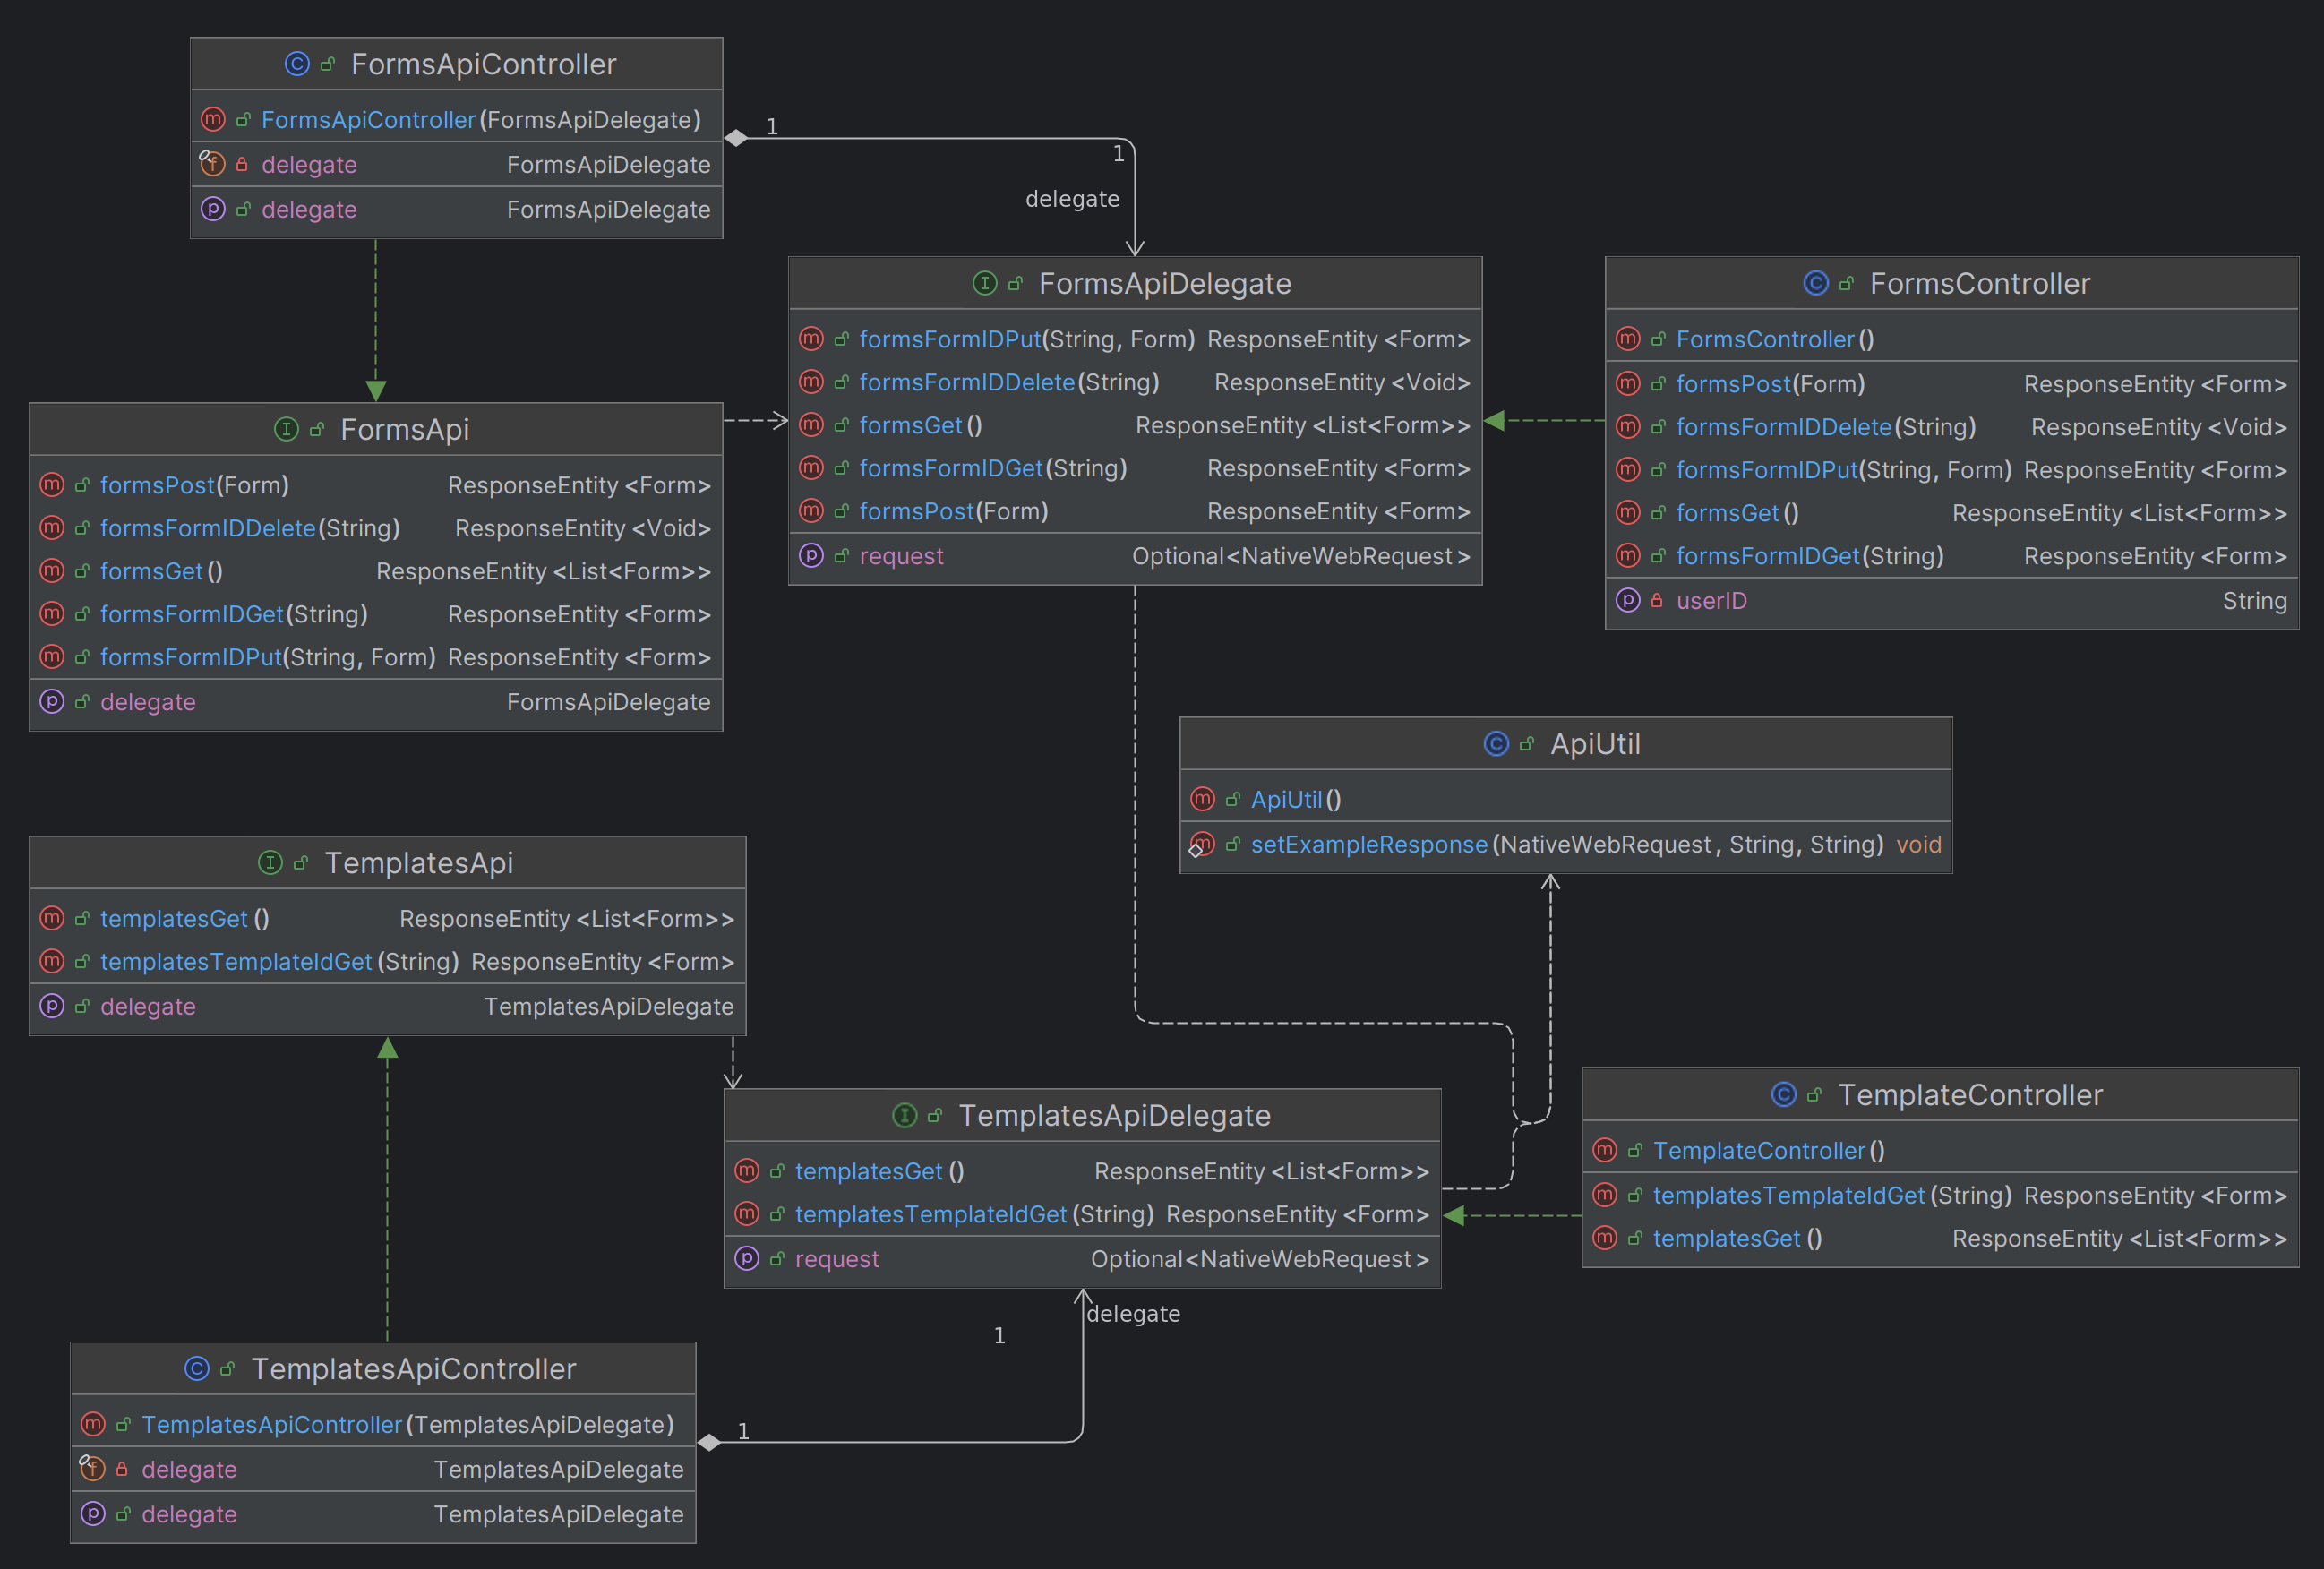
\includegraphics[width=15cm]{images/classDiagrams/Api}
    \caption{Backend API Controller}\label{fig:Backend-API-Controller}
\end{figure}

Die Implementierung der \ac{API} Endpunkte erfolgt in den jeweiligen Controllern.
Diese verwenden generierte Interfaces, wie in \refa{fig:Backend-API-Controller} zu sehen ist.

% \subsection{Frontend}
% Irgendwie Unhappy damit
% Finde Beim Frontend Derzeit nichts Sinfolles

\section{Verhaltensschicht}\label{sec:verhaltensschicht}
Im Folgenden wird das Verhalten der Applikation exemplarisch bei den Usecases Ausfüllen 
eines Antrags, sowie Login beschrieben.

\begin{figure}[H]
    \includegraphics[width=15cm, height=19cm]{Doc/images/Fill_in_Form_Sequence_Diagramm_part 1.png}
    \caption{Antrag ausfüllen Diagramm Teil 1}\label{fig:Antrag Flow 1}
\end{figure}   
\begin{figure}[H]
    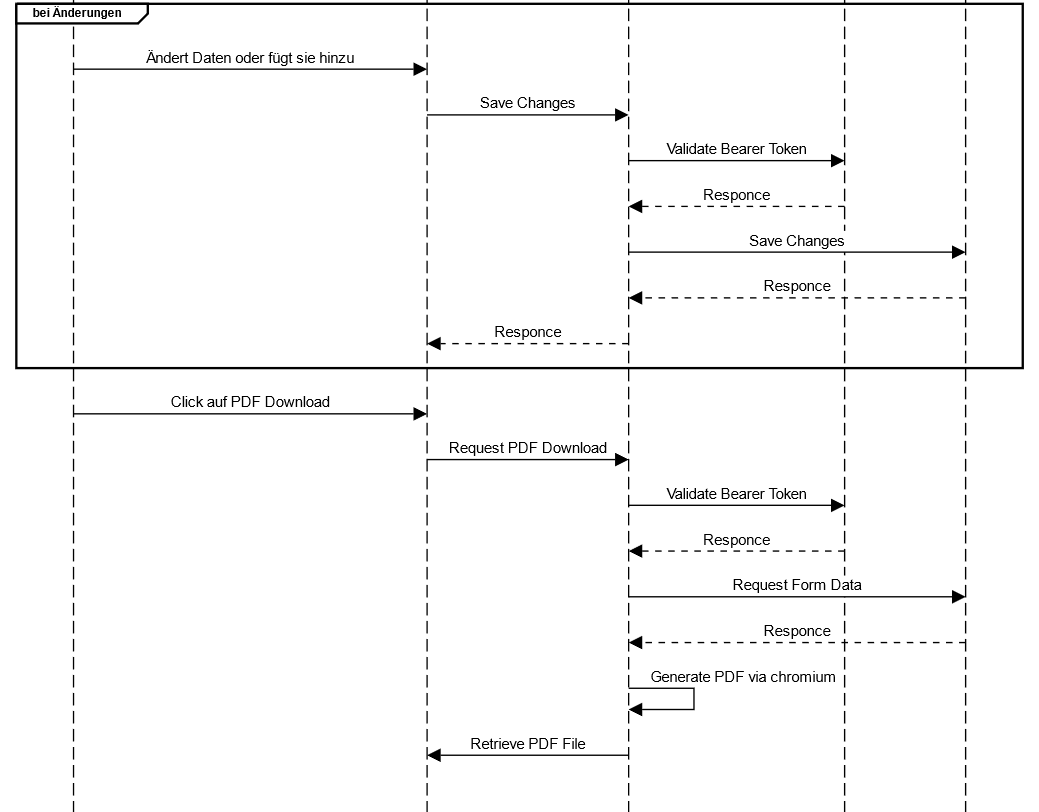
\includegraphics[width=15cm]{Doc/images/Fill_in_Form_Sequence_Diagramm_part_2.png}
    \caption{Antrag ausfüllen Sequence Diagramm Teil 2}\label{fig:Antrag Flow 2}
\end{figure}
\refa{fig:Antrag Flow 1} und \refa{fig:Antrag Flow 2} zeigen den sequenziellen Ablauf 
und die Interaktionen, die Ablaufen, wenn der Nutzer einen Antrag ausfüllt und dabei 
gegebenenfalls diverse Features wie die Autofill Funktion nutzt.
\begin{figure}[H]
    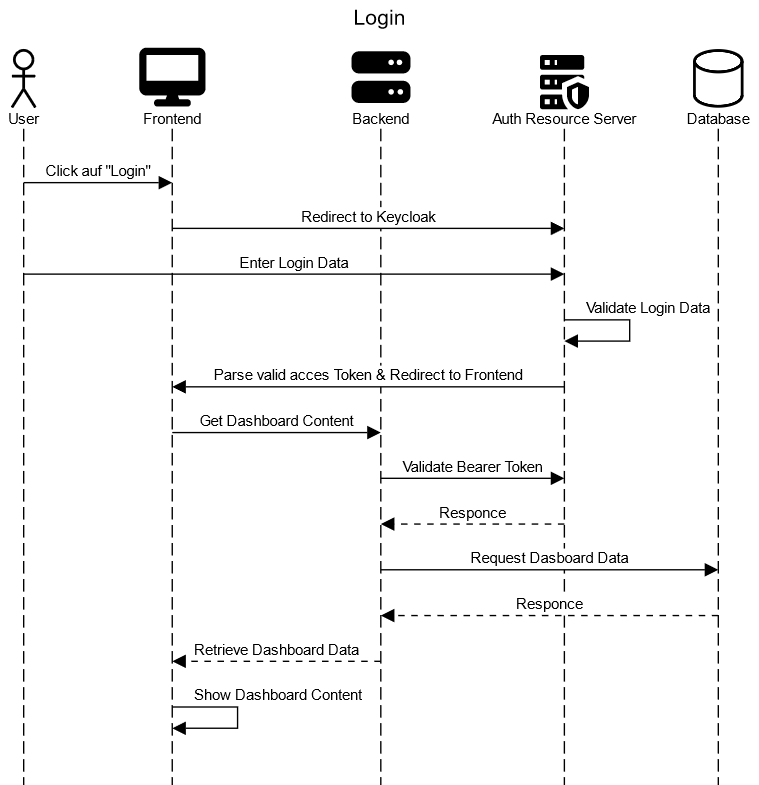
\includegraphics[width=15cm]{Doc/images/Login.png}
    \caption{Login Sequence Diagramm}\label{fig:Login Flow}
\end{figure}
\refa{fig:Login Flow} zeigt, wie die Applikation eine Authentifizierung des Nutzers und damit 
eine Login-Funktionalität ermöglicht, bzw. wie diese umgesetzt wird.

\section{Verteilungsschicht}\label{sec:verteilungsschicht}
Die Applikation verteilt sich, wie \refa{fig:Netzwerksuebersicht} zeigt, auf drei frei verfügbare Komponenten.
Ein Nutzer kann über die Subdomains "df." für das Frontend, "backend.df." für das Backend und "auth.df."
auf die Komponenten zugreifen.
Das Backend sowie der Authentifizierungsdienst verfügen jeweils zusätzlich über eine lokal verfügbare Datenbank.

\begin{figure}[h]
    \centering
    \includesvg[width=14cm]{./images/GeneralNetwork}
    \caption{Netzwerksübersicht}\label{fig:Netzwerksuebersicht}
\end{figure}

\newpage
\refa{fig:Container-verteilung} zeigt, wie die Anwendung auf einem Server bereitgestellt werden kann.
Dies stellt ebenfalls den Aufbau des verwendeten \ac{CD} Servers dar.
Dieses Projekt stellt die Docker Compose (dargestellt links in \refa{fig:Container-verteilung})
sowie die darin enthaltenen Container zur Verfügung.

Der rechte Teil von \refa{fig:Container-verteilung} empfiehlt die Verwendung von Traefik\footnote{https://traefik.io/traefik/}
als Reverse Proxy.
Die Verwendung eines Reverse Proxy bringt verschiedene Vorteile:
\begin{itemize}
    \item Automatische Redirects von http auf https
    \item Zentrale Absicherung der Dienste mit \ac{SSL}-Verschlüsselung
    \item Routen der Dienste basierend auf deren Subdomain
\end{itemize}

\begin{figure}[h]
    \centering
    \includesvg[width=17cm]{images/ServerSetup}
    \caption{Container verteilung}\label{fig:Container-verteilung}
\end{figure}